% This is samplepaper.tex, a sample chapter demonstrating the
% LLNCS macro package for Springer Computer Science proceedings;
% Version 2.20 of 2017/10/04
\documentclass[runningheads]{llncs}
%
\usepackage{graphicx}

\begin{document}
%
\title{Smart Library}

\author{Group25, Bhagyalaxmi \and
Divya \and
Jerome}

\institute{Service Computing Department, IAAS, University of Stuttgart
\email{st164379@stud.uni-stuttgart.de} 
\newline\email{st164388@stud.uni-stuttgart.de} 
\newline\email{st1164430@stud.uni-stuttgart.de}}
%
\maketitle              % typeset the header of the contribution
%

\section{Introduction}
Smartness can be established in any sector of the urban area: be it in an office, school, transportation infrastructure, library etc. Our idea is centralized to a library with focus on energy consumption, security, safety and comfort of its occupants. 
Energy consumption can be controlled prudently by handling the lighting system, HVAC and other electronic components dynamically. Security is obtained by the alarming system in case of unexpected and malicious entry into the environment under consideration. 
Sensors and actuators are combined to provide the desired outcome here.

\section{Requirements specification}
%
\begin{enumerate}
\item\textbf{Presence Based Lighting Control:}
The automatic lighting control in our context refers to turning on and off the lights depending on the presence of subjects in the environment. A light sensor is used to detect and adjust the brightness in the room depending on the amount of the light available in the surrounding. Energy gets saved in these scenarios.

\item\textbf{Occupancy Prediction:}
The number of occupants in the building is detected and stored for every fixed interval of time. (Ex. Monday 9:00 to 9:15 Number of Occupants = 20). The data is stored in the cloud repository. After receiving at least a week’s data the occupancy prediction is made for the next week based on this data. The prediction algorithm is a simple average of the past number of occupants at that time interval. 

\item\textbf{HVAC System Control Based on local sensors and Weather forecast:}
User desired temperature is taken as input. Temperature Sensor is used to get the real time values. Weather forecast is used to predict the outside temperature changes in the next hour from then. The heating and cooling system is switched on and off based on the difference in the temperatures observed between the library and the surroundings. The Weather forecast and the occupancy prediction is also taken into consideration of the HVAC control.

\item\textbf{Burglar Alarm System:}
PIR sensors and library timings are used to detect suspicious entry into the building in unexpected times. Once these suspicious movements are detected, a notification is sent to the responsible alerting the situation.
\end{enumerate}

\section{System architecture}
Fig \ref{fig1} gives the System architecture of Smart Library.
\begin{figure}
\begin{center}
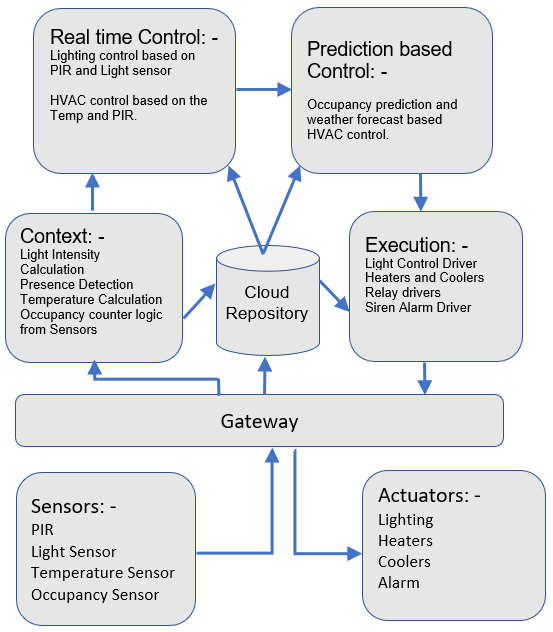
\includegraphics[height=10cm, width=10cm]{fig1}
\caption{System Architecture} \label{fig1}
\end{center}
\end{figure}

\section{Conclusions and Outlook}
By this implementation, we intend to bring energy efficiency in the library with security, comfort and safety to the user thus fulfilling the purpose of a smart city to an extent utilizing the internet of things technology.

\end{document}
